\documentclass[final,a4paper]{article}
\usepackage[ngerman]{babel}
\usepackage[utf8]{inputenc}
\usepackage[T1]{fontenc}
\usepackage{lmodern}
\usepackage{listings}
\usepackage{graphicx}

\begin{document}
\lstset{tabsize=4}
\lstset{basicstyle=\small}
\lstset{language=java}

{\huge Programmiervorkurs Tag 2 - Aufgaben}

\bigskip

\begin{enumerate}
\item{
	Welchen booleschen Wert ergeben die folgenden Ausdrücke:
	\begin{itemize}
		\item \lstinline{true & false}
		\item \lstinline{true & true}
		\item \lstinline{false & false}
		\item \lstinline{false | false}
		\item \lstinline{false | true}
		\item \lstinline{true | true}
		\item \lstinline{false ^ false}
		\item \lstinline{true ^ false}
		\item \lstinline{true ^ true}
		\item \lstinline{true & !true}
		\item \lstinline{(true | false) & (false | (true & true & true | false)) | !false}
		\item \lstinline{1 == 2 && (3 != 4) || (1 < 2)}
		\item \lstinline{(7 < 5) ^ (2 == (9 / 4))}
	\end{itemize}
}

\item{
Welche der folgenden Aussagen sind richtig
\begin{itemize}
\item Wenn \lstinline{(a || b)} true ist, ist mindestens eine der Variablen true.
\item Wenn \lstinline{(a && b)} true ist, sind beide Variablen true.
\item Wenn \lstinline{(a && b)} false ist, sind beide Variablen false.
\item Wenn \lstinline{(a || b)} false ist, sind beide Variablen false.
\item Wenn \lstinline{!(a && b)} false ist, ist keine der beiden Variablen true.
\item Wenn \lstinline{ !(a || b)} false ist, sind beide Variablen true.
\item \lstinline{(a && b) || !(a && b)} ist immer true.
\end{itemize}
}

\item{
Gib eine Bedingung an, die für einen int-Wert x wahr wird, wenn dieser über 25 liegt und eine ungerade Zahl ist. (Lösungshinweis:  Zur Prüfung, ob es sich um eine ungerade Zahl handelt, ist der Modulo-Operator \% hilfreich.)

}

\item{
Ein Schaltjahr ist ein Jahr, dessen Jahreszahl restlos durch vier teilbar ist. Eine Ausnahme bilden die vollen Jahrhundertjahre, deren Jahreszahl durch 100 teilbar ist: Diese sind nur dann ein Schaltjahr, wenn ihre Jahreszahl auch durch 400 teilbar ist.
Gib einen booleschen Ausdruck an, der für einen Integer-Wert jahr genau dann wahr wird, wenn es sich bei dem in jahr gespeicherten Wert um die Jahreszahl eines Schaltjahrs handelt.
}

\item{
Ändere das folgende Programm so, dass es Frauen und Männer bei der Begrüßung unterscheidet:
\begin{lstlisting}
	boolean male = true;
	String name = "Peter";
	
	System.out.println("Guten Tag, Herr " + name);
\end{lstlisting}
}

\item{
Mit Hilfe der p-q-Formel lassen sich quadratische Gleichungen der Form \(x^2 + p \cdot x + q = 0\) lösen. Es gilt: \(x_{1/2} = - \frac{p}{2} \pm \sqrt{\left( \frac{p}{2}\right)^2 -q}\). Eine reelle Lösung existiert nur dann, wenn die Diskriminante (der Ausdruck unter der Wurzel) nicht negativ ist. 

Schreibe ein Programm, das das Ergebnis/die Ergebnisse für gegebene p und q berechnet und auf der Konsole ausgibt. Wenn es kein Ergebnis im Bereich der reellen Zahlen gibt, soll eine entsprechende Meldung auf der Konsole ausgegeben werden. 

Um Wurzeln und Potenzen zu berechnen, kannst du die Methoden sqrt()/Sqrt() und pow()/Pow() der Klasse Math verwenden. Beide Methoden nehmen double-Werte als Parameter entgegen und geben einen double-Wert zurück, den man zum Beispiel in einer Variablen speichern kann.

Bsp.: 
\begin{itemize}
\item Math.sqrt(4.0) gibt den Wert 2.0 zurück
\item Math.pow(2.0, 3.0) gibt den Wert 8.0 zurück
\end{itemize}

}

\item{
Schreibe ein Programm, das abhängig von einem Winkel (positiver Integer-Wert) eine der vier Himmelsrichtung Norden, Osten, Süden oder Westen ausgibt. Norden liegt dabei auf \(0^\circ\). 

Es reicht, wenn Winkel von \(0^\circ\) bis \(359^\circ\) verarbeitet werden können.
}

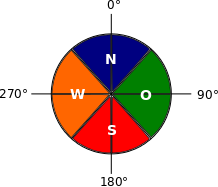
\includegraphics{aufgabe_2_7_kompass.png}

\item{
Schreibe ein Programm, das das gleiche Ziel ganz ohne if-Abfragen nur mit switch/case erreicht.

Lösungshinweise: Normiere den Winkelbereich auf die Anzahl der Himmelsrichtungen. Jede Himmelsrichtung wird dann durch einen von vier Integer-Werten repräsentiert, der als Switch-Variable dient. Dabei ist die ganzzahlige Division hilfreich.

Du solltest dir außerdem überlegen, was man gegen die „unschöne“ Aufteilung der Winkelbereiche tun kann. Jeder dieser Bereiche ist zwar \(90^\circ\) groß, aber Norden liegt zum Beispiel zwischen \(315^\circ\) und \(45^\circ\), Süden zwischen \(135^\circ\) und \(225^\circ\). Das ist zum Normieren etwas unpraktisch.
}
\end{enumerate}
\end{document}